\documentclass[tikz,border=10pt]{standalone}
% Shared look for every TikZ diagram. Load with % Shared look for every TikZ diagram. Load with % Shared look for every TikZ diagram. Load with \input{../../tools/tikz-style.tex}
\usepackage[T1]{fontenc}
\usepackage{lmodern}
\renewcommand{\sfdefault}{lmr}  % diagrams use the same serif as the text
\usetikzlibrary{arrows.meta, positioning, shapes.geometric, calc, fit, backgrounds}
\definecolor{cblue}{HTML}{4C78A8}
\definecolor{corange}{HTML}{F58518}
\definecolor{cgreen}{HTML}{54A24B}
\definecolor{cred}{HTML}{E45756}
\definecolor{cpurple}{HTML}{B279A2}
\definecolor{cgrey}{HTML}{6B6B6B}
\tikzset{
  every picture/.style={font=\sffamily, line width=1.2pt},
  box/.style={draw=#1, fill=#1!12, rounded corners=4pt, align=center, inner sep=7pt, minimum height=1.1cm},
  box/.default=cgrey,
  arrow/.style={-{Stealth[length=3mm]}, draw=cgrey, line width=1.4pt},
  title/.style={font=\sffamily\bfseries\Large},
  note/.style={font=\sffamily\small, text=cgrey, align=center},
}
\AtBeginDocument{\hyphenpenalty=10000 \exhyphenpenalty=10000}

\usepackage[T1]{fontenc}
\usepackage{lmodern}
\renewcommand{\sfdefault}{lmr}  % diagrams use the same serif as the text
\usetikzlibrary{arrows.meta, positioning, shapes.geometric, calc, fit, backgrounds}
\definecolor{cblue}{HTML}{4C78A8}
\definecolor{corange}{HTML}{F58518}
\definecolor{cgreen}{HTML}{54A24B}
\definecolor{cred}{HTML}{E45756}
\definecolor{cpurple}{HTML}{B279A2}
\definecolor{cgrey}{HTML}{6B6B6B}
\tikzset{
  every picture/.style={font=\sffamily, line width=1.2pt},
  box/.style={draw=#1, fill=#1!12, rounded corners=4pt, align=center, inner sep=7pt, minimum height=1.1cm},
  box/.default=cgrey,
  arrow/.style={-{Stealth[length=3mm]}, draw=cgrey, line width=1.4pt},
  title/.style={font=\sffamily\bfseries\Large},
  note/.style={font=\sffamily\small, text=cgrey, align=center},
}
\AtBeginDocument{\hyphenpenalty=10000 \exhyphenpenalty=10000}

\usepackage[T1]{fontenc}
\usepackage{lmodern}
\renewcommand{\sfdefault}{lmr}  % diagrams use the same serif as the text
\usetikzlibrary{arrows.meta, positioning, shapes.geometric, calc, fit, backgrounds}
\definecolor{cblue}{HTML}{4C78A8}
\definecolor{corange}{HTML}{F58518}
\definecolor{cgreen}{HTML}{54A24B}
\definecolor{cred}{HTML}{E45756}
\definecolor{cpurple}{HTML}{B279A2}
\definecolor{cgrey}{HTML}{6B6B6B}
\tikzset{
  every picture/.style={font=\sffamily, line width=1.2pt},
  box/.style={draw=#1, fill=#1!12, rounded corners=4pt, align=center, inner sep=7pt, minimum height=1.1cm},
  box/.default=cgrey,
  arrow/.style={-{Stealth[length=3mm]}, draw=cgrey, line width=1.4pt},
  title/.style={font=\sffamily\bfseries\Large},
  note/.style={font=\sffamily\small, text=cgrey, align=center},
}
\AtBeginDocument{\hyphenpenalty=10000 \exhyphenpenalty=10000}

\begin{document}
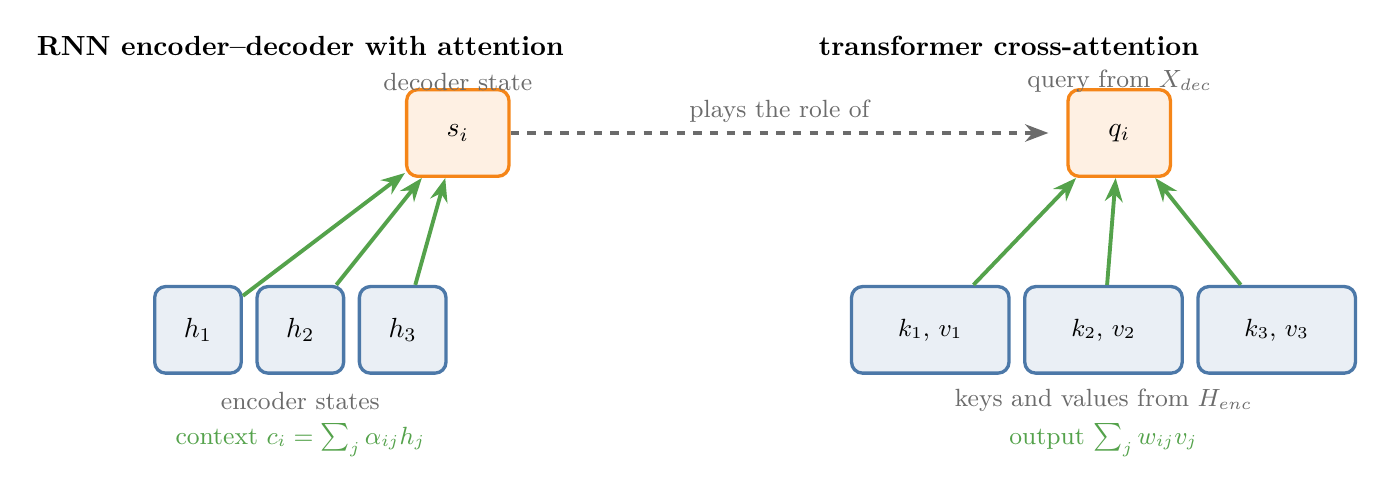
\begin{tikzpicture}[h/.style={box=cblue, minimum width=1.1cm, font=\sffamily}, s/.style={box=corange, minimum width=1.3cm, font=\sffamily}]
  \node[font=\sffamily\bfseries] at (2.6,3.6) {RNN encoder–decoder with attention};
  \foreach \j in {1,2,3} \node[h] (h\j) at (1.3*\j,0) {$h_\j$};
  \node[s] (s) at (4.6,2.5) {$s_i$};
  \foreach \j in {1,2,3} \draw[arrow, draw=cgreen] (h\j) -- (s);
  \node[note, text=cgreen] at (2.6,-1.4) {context $c_i = \sum_j \alpha_{ij} h_j$};
  \node[note] at (2.6,-0.9) {encoder states};
  \node[note] at (4.6,3.15) {decoder state};
  \node[font=\sffamily\bfseries] at (11.6,3.6) {transformer cross-attention};
  \foreach \j in {1,2,3} \node[h, minimum width=2.0cm, font=\sffamily\small] (k\j) at (8.4+2.2*\j,0) {$k_\j$, $v_\j$};
  \node[s] (q) at (13.0,2.5) {$q_i$};
  \foreach \j in {1,2,3} \draw[arrow, draw=cgreen] (k\j) -- (q);
  \node[note] at (12.8,-0.9) {keys and values from $H_{enc}$};
  \node[note, text=cgreen] at (12.8,-1.4) {output $\sum_j w_{ij} v_j$};
  \node[note] at (13.0,3.15) {query from $X_{dec}$};
  \draw[dashed, cgrey, -{Stealth}] (s.east) -- node[above, note] {plays the role of} (12.1,2.5);
  \end{tikzpicture}
\end{document}
